\definecolor{ttttff}{rgb}{0.2,0.2,1}

%dash pattern=on 5pt off 2pt
%[fill = white, rounded corners = 5pt, inner sep=0.8pt]
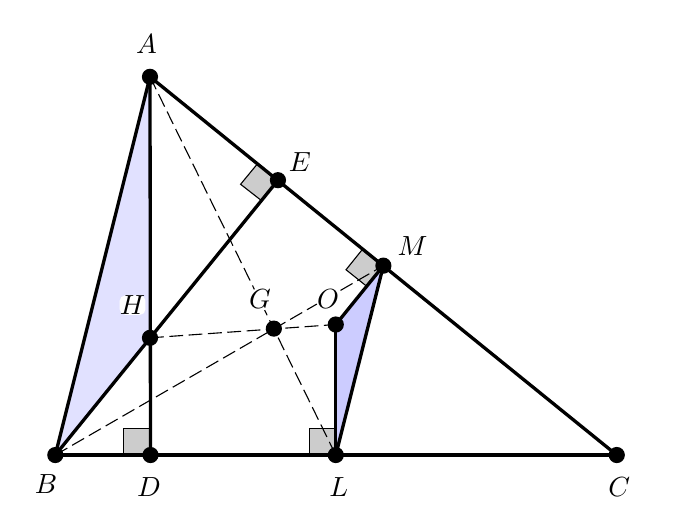
\begin{tikzpicture}[scale = 0.65]
    \clip(-2.17,-2.6) rectangle (9.95,6.67);
    \draw[line width=0.4pt,fill=black,fill opacity=0.2] (2.32,4.01) -- (1.99,3.61) -- (2.4,3.29) -- (2.72,3.69) -- cycle;
    \draw[line width=0.4pt,fill=black,fill opacity=0.2] (0.23,-1.16) -- (-0.29,-1.16) -- (-0.29,-1.68) -- (0.23,-1.68) -- cycle;
    \draw[line width=0.4pt,fill=black,fill opacity=0.2] (4.38,2.35) -- (4.05,1.94) -- (4.45,1.62) -- (4.78,2.02) -- cycle;
    \draw[line width=0.4pt,fill=black,fill opacity=0.2] (3.85,-1.16) -- (3.34,-1.16) -- (3.34,-1.68) -- (3.85,-1.68) -- cycle;
    \fill[line width=0pt,color=ttttff,fill=ttttff,fill opacity=0.15] (-1.63,-1.68) -- (0.22,5.71) -- (0.22,0.61) -- cycle;
    \fill[line width=0pt,color=ttttff,fill=ttttff,fill opacity=0.25] (4.78,2.02) -- (3.85,0.87) -- (3.85,-1.68) -- cycle;
    \draw [line width=1.2pt] (-1.63,-1.68)-- (9.34,-1.68);
    \draw [line width=1.2pt] (0.22,5.71)-- (9.34,-1.68);
    \draw [line width=1.2pt] (0.22,5.71)-- (-1.63,-1.68);
    \draw [line width=1.2pt] (0.22,5.71)-- (0.23,-1.68);
    \draw [line width=1.2pt] (-1.63,-1.68)-- (2.72,3.69);
    \draw [line width=1.2pt] (3.85,-1.68)-- (3.85,0.87);
    \draw [line width=1.2pt] (4.78,2.02)-- (3.85,0.87);
    \draw [line width=1.2pt] (3.85,-1.68)-- (4.78,2.02);
    \draw [dash pattern=on 5pt off 2pt] (0.22,5.71)-- (3.85,-1.68);
    \draw [dash pattern=on 5pt off 2pt] (-1.63,-1.68)-- (4.78,2.02);
    \draw [dash pattern=on 5pt off 2pt] (0.22,0.61)-- (3.85,0.87);
    \begin{scriptsize}
        \normalsize
        \fill [color=black] (0.22,5.71) circle (4.5pt);
        \draw[color=black] (0.15,6.35) node[fill = white, rounded corners = 5pt, inner sep=0.8pt] {$A$};
        \fill [color=black] (-1.63,-1.68) circle (4.5pt);
        \draw[color=black] (-1.81,-2.25) node[fill = white, rounded corners = 5pt, inner sep=0.8pt] {$B$};
        \fill [color=black] (9.34,-1.68) circle (4.5pt);
        \draw[color=black] (9.39,-2.3) node[fill = white, rounded corners = 5pt, inner sep=0.8pt] {$C$};
        \fill [color=black] (0.23,-1.68) circle (4.5pt);
        \draw[color=black] (0.2,-2.3) node[fill = white, rounded corners = 5pt, inner sep=0.8pt] {$D$};
        \fill [color=black] (2.72,3.69) circle (4.5pt);
        \draw[color=black] (3.15,4.05) node[fill = white, rounded corners = 5pt, inner sep=0.8pt] {$E$};
        \fill [color=black] (4.78,2.02) circle (4.5pt);
        \draw[color=black] (5.35,2.4) node[fill = white, rounded corners = 5pt, inner sep=0.8pt] {$M$};
        \fill [color=black] (3.85,-1.68) circle (4.5pt);
        \draw[color=black] (3.91,-2.3) node[fill = white, rounded corners = 5pt, inner sep=0.8pt] {$L$};
        \fill [color=black] (3.85,0.87) circle (4.5pt);
        \draw[color=black] (3.7,1.36) node[fill = white, rounded corners = 5pt, inner sep=0.8pt] {$O$};
        \fill [color=black] (0.22,0.61) circle (4.5pt);
        \draw[color=black] (-0.12,1.25) node[fill = white, rounded corners = 2pt, inner sep=0.1pt] {$H$};
        \fill [color=black] (2.64,0.79) circle (4.5pt);
        \draw[color=black] (2.37,1.36) node[fill = white, rounded corners = 5pt, inner sep=0.8pt] {$G$};
    \end{scriptsize}
\end{tikzpicture}